\documentclass[11pt,a4paper]{article}
\usepackage[utf8]{inputenc}

\usepackage{graphicx}
\graphicspath{{images/}}
\usepackage[dvipsnames]{xcolor}

%\usepackage[paper=a4paper]{geometry}
\usepackage{longtable}
\usepackage{rotating}


\usepackage[final]{pdfpages}
\usepackage{float}

\usepackage{listings}

\usepackage{color}
\definecolor{gray}{rgb}{0.4,0.4,0.4}
\definecolor{lightgray}{rgb}{0.9,0.9,0.9}
\definecolor{darkblue}{rgb}{0.0,0.0,0.6}
\definecolor{cyan}{rgb}{0.0,0.6,0.6}

\lstset{
  basicstyle=\ttfamily,
  columns=fullflexible,
  showstringspaces=false,
  backgroundcolor=\color{lightgray},
  tabsize=3,
  breaklines=true,
  breakatwhitespace=true,
  commentstyle=\color{gray}\upshape
}

\lstdefinelanguage{XML}
{
  morestring=[b]",
  morestring=[s]{>}{<},
  morecomment=[s]{<?}{?>},
  stringstyle=\color{black},
  identifierstyle=\color{darkblue},
  keywordstyle=\color{cyan},
  morekeywords={xmlns,version,type}% list your attributes here
}


\begin{document}
\begin{titlepage}
\centering
%\newgeometry{top=3in,bottom=1in,right=1.0in,left=1.0in}
\huge The Project Game \\
\vspace{1.5cm}
\large Kamil Grabowski, Filip Grajek, Bartosz Jasiński, Ivan Rukhavets \\
\vspace{1.0cm}
Wersja 1.0 \\
\vspace{1.0cm}
\today
\end{titlepage}

\center{\Large{\textrm{Wydział Matematyki i Nauk Informacyjnych Politechniki Warszawskiej}}}
		
\begin{figure}
	\centering
\includegraphics[scale=0.3]{images/logo.png}
\end{figure}	
\newpage
			
\begin{longtable}{| l | p{4.5cm} | p{4.5cm} | l | }
\hline
\textbf{Date} & \textbf{Author} & \textbf{Description} & Version \\ \hline
15.10.2016 & Kamil Grabowski, Filip Grajek, Bartosz Jasiński, Ivan Rukhavets & Initial document & 1.0 \\ \hline
\end{longtable}

\tableofcontents

\section{Introduction}

\section{Requirements}

\subsection{Functional requirements}

\begin{figure}[H]
\begin{center}
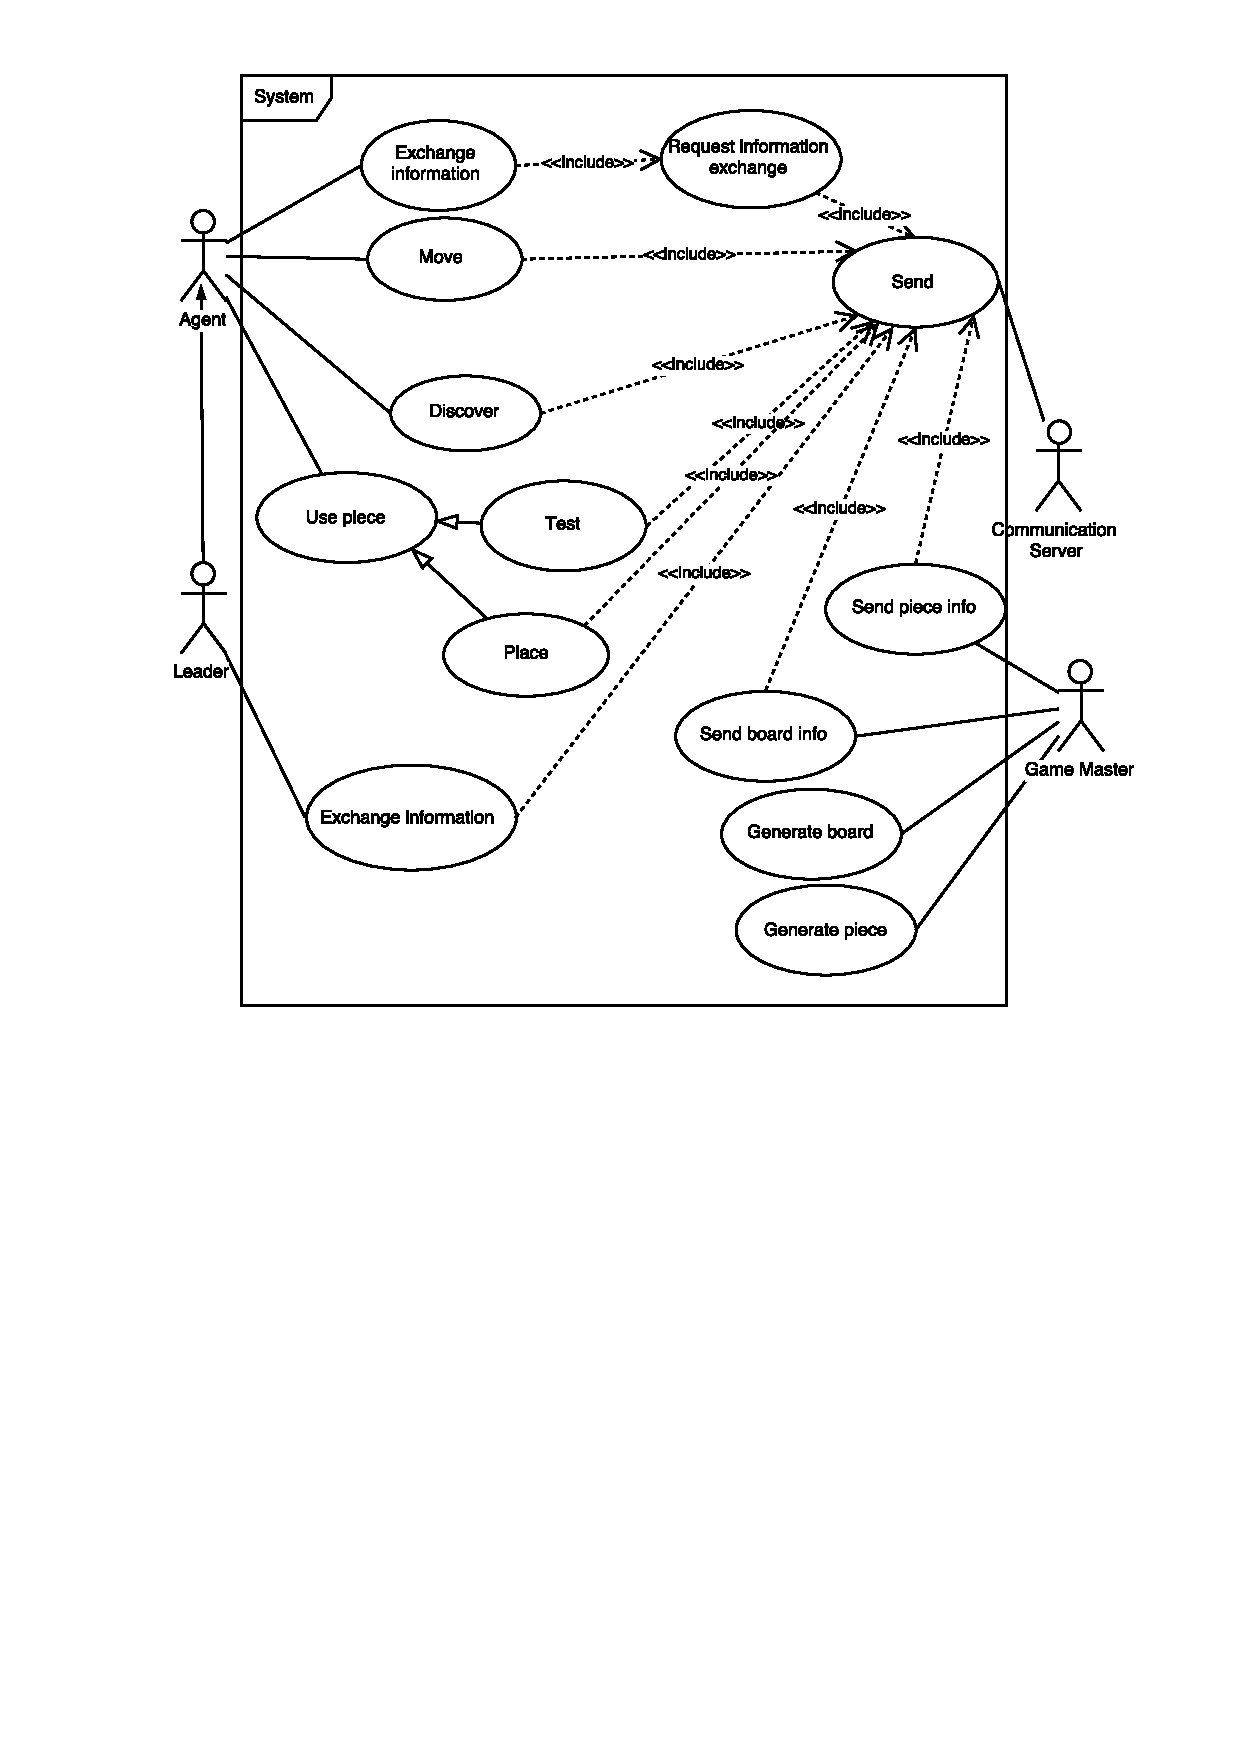
\includegraphics[trim={2cm 10cm 0 0},clip, scale=0.7]{UseCases}
\caption{Use-case diagram}
\end{center}
\end{figure}

In the system there will be four main actors:
\begin{enumerate}
\item Game Master
\item Agents
\item Team Leaders
\item Communication Server
\end{enumerate}
The game master is the core of the system. At the start he will generate the board and the first pieces. He is also responsible for managing the board and sending information to the agents during the game, for example he will decide if a move is possible. Because the game master is the only part of the system which knows the exact state of the board, he also has to inform the agents when a team has won. \\
An agent is an independent program that collaborates with other agents from his team in order to complete the project first. He is able to move on the board, during movement he discovers the state of the board around him. If he walks on a field with a piece, he will collect it and then he can test it or place it in his goal area. All those actions have to be passed to the game master, since he decides the outcome of it.  An agent is also able to request an information exchange with other agents. If the request is accepted, both agents share their current board state.\\
The team leaders are two special agents (one in each team), so they have the same functionality as an agent.Moreover, they can exchange information directly with other agents, without having to ask first. \\
The agents and the game master are all independent programs, they could be even on different computers. Because of that, we need a communication server. It has only one responsibility: passing messages between all parts of the system.
\subsection{Non-functional requirements}

\begin{longtable}{| p{3.5cm} | l | p{5.5cm} |}
\hline
\textbf{Requirement class} & Requirement number & Description \\ \hline
\textbf{Usability} & 1 & A Read-me file will be added with an instruction how to setup the system. \\ \hline
\textbf{Reliability} & 2 & The system will continue to work properly even when one or more agents disconnect unexpectedly. \\ \hline
\textbf{Performance} & - & There are no requirements in this class. \\ \hline
\textbf{Supportability} & 3 & The application logic will be tested using unit tests.\\ \cline{2-3}
 & 4 & Configuration will be possible through a configuration file.\\ \hline
\end{longtable}

\subsection{Runtime parameters}


We have decided to make configuration possible through the game master before starting a game. The player can choose a graphical user interface or a configuration file to do this. When making changes in the menu, the file is automatically overwritten (through xml serialization) to save the settings. When starting a new game, the configuration is always parsed from the file. This way the game parameters are always saved and can easily be exported. \\
The configuration file will be a xml file, as those types of files are readable by humans and programs. Moreover, through the use of xml schemes we can validate such a file without problems. \\
The parameters specified in the configuration file are:
\begin{enumerate}
\item Board size
\item Task area size
\item Minimum number of players per team
\item Maximum number of players per team
\item Ip address and port of the communication server
\item Number of tasks to complete for victory
\end{enumerate}
If the need arises, new parameters can be added to the file without any problems (like backwards compatibility), which is another advantage of using xml.

\section{Design documentation}

\subsection{Architecture}

\begin{figure}
\begin{center}
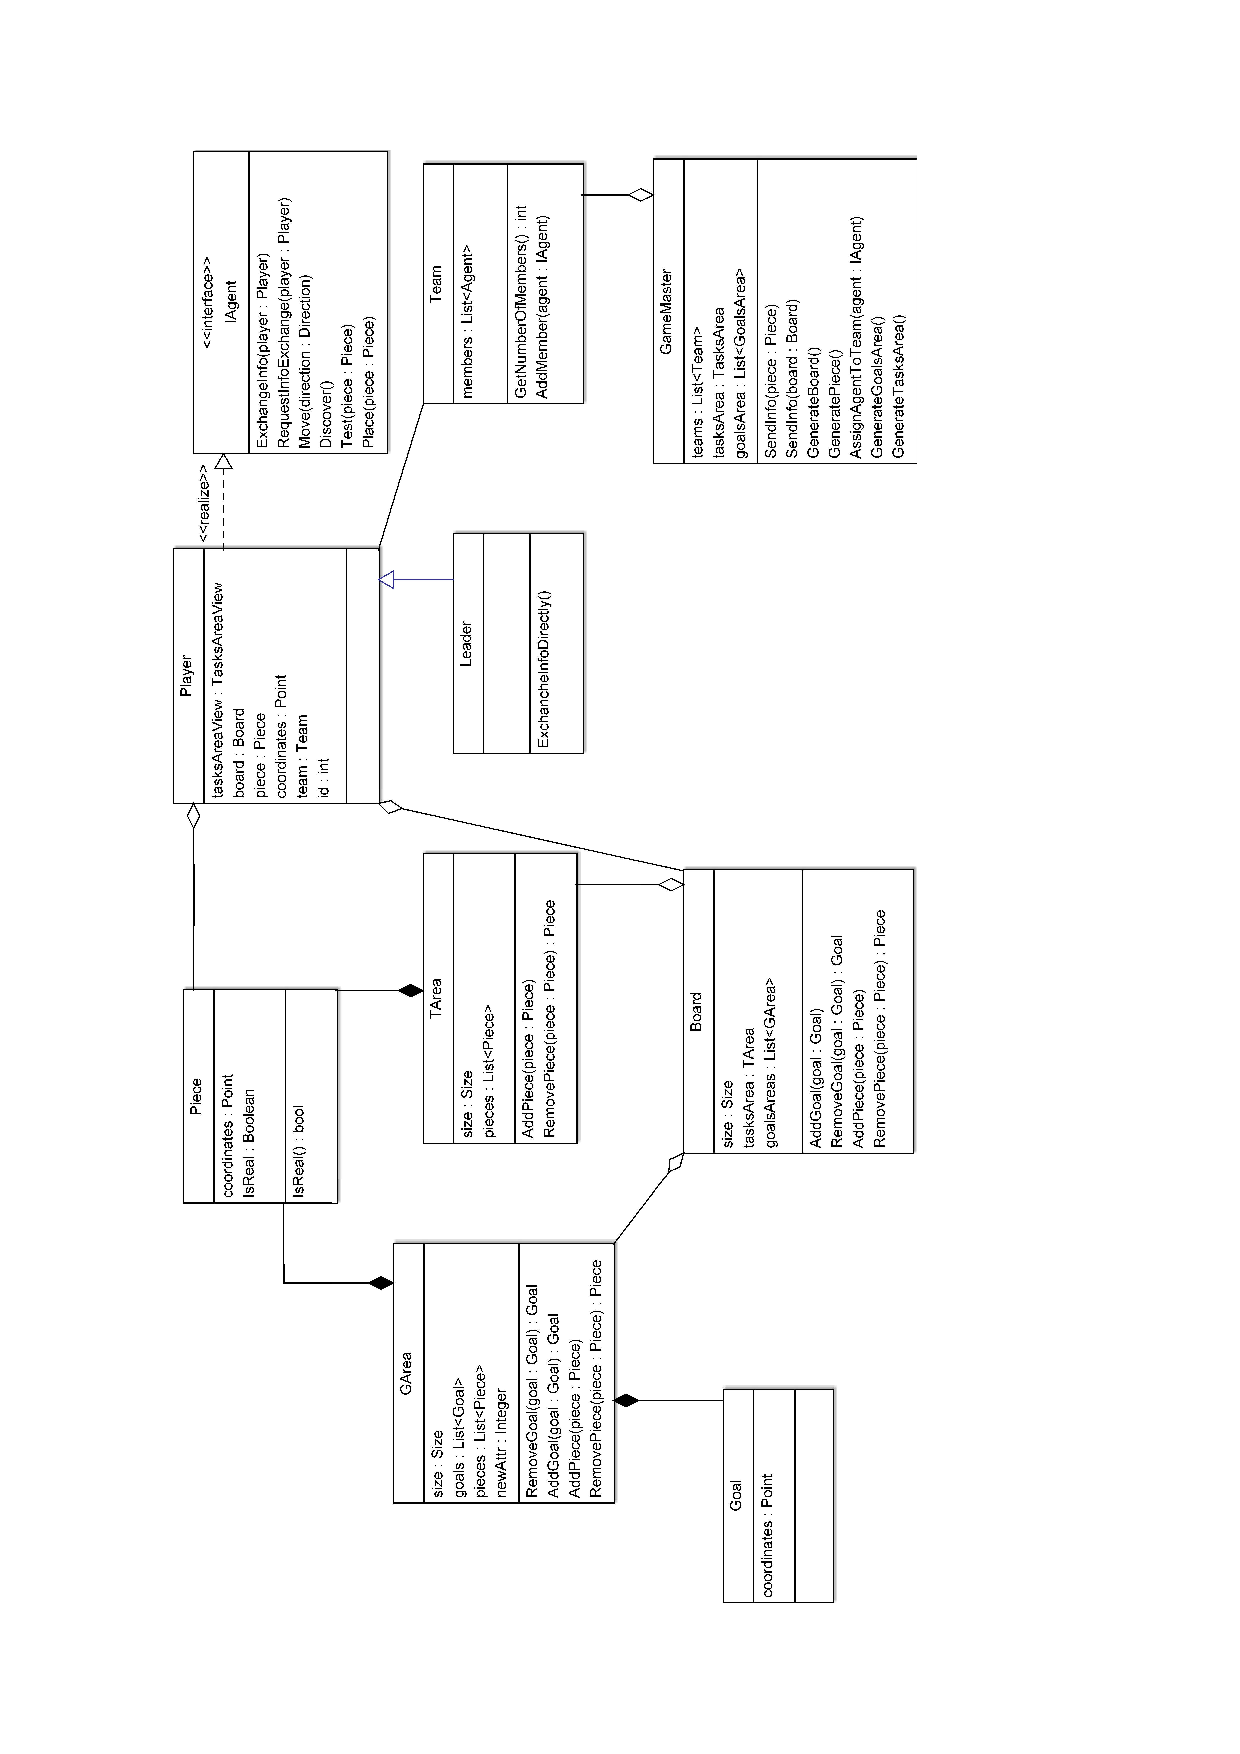
\includegraphics[scale=0.7]{architecture}
\caption{Architecture of system}
\end{center}
\end{figure}

Game Project architecture consists of fourn main building blocks:
\begin{itemize}
\item Game Area
\item Agents
\item Game Master
\item Server
\end{itemize}

which respectively has folowing components\\
\cdot Game Area:
\begin{itemize}
\item GArea - area consising game targets which agents have cover with pieces in order to win the game.
\item TArea - area consising pieces which agents raises in order to move them to goal area.
\item Board - class which represents board consists one TArea and list of GAreas
\end{itemize}

\cdot Agents:
\begin{itemize}
\item IAgent - interface for agents, it has basic agent methods
\item Player - class which implements IAgent, represents usual agents in game
\item Leader - class which has additional methods characteristic for team leader
\item Team - class which holds team members useful for communication
\end{itemize}

\cdot Game Master:
\begin{itemize}
\item Game Master - class which represents object managing the entire game.
\end{itemize}

\cdot Server:
\begin{itemize}
\item Server - server of the game its only purpose is to exchange messages between Agents and Game Master
\end{itemize}

\subsection{Messages}

\subsubsection{Game initiation}

After connecting to the communication server, the agent gets a list of games he can join. In order to choose a game, he has to send a message, defined by the following schema:
\lstinputlisting[language=XML]{xml/gameConnect.xsd}
Here is a example of such a message, an agent wants to join the first team in the game with id zero:
\lstinputlisting[language=XML]{xml/gameConnect.xml}

\subsubsection{Gameplay}
Before making every move, agent sends a message with its description to the server. The message is defined by following schema:
\lstinputlisting[language=XML]{xml/move.xsd}

Here is an example of moving up of agent with id 10:
\lstinputlisting[language=XML]{xml/move-up.xml}

And here is a message sent by agent with id 007 when it wants to request information with agent 10: 
\lstinputlisting[language=XML]{xml/move-exchange.xml}

As an answer agent gets message from server described with that schema:
\lstinputlisting[language=XML]{xml/serverResponceOnMove.xsd}
It tells if it allows for move and optionaly sends information from another agent with distance from each known field to a piece.
For example:
\lstinputlisting[language=XML]{xml/serverResponceOnMove.xml}

After the game is finished, server sends information to all agents about game results with following schema(example attached).
\lstinputlisting[language=XML]{xml/gameEnd.xsd}
\lstinputlisting[language=XML]{xml/gameEnd.xml}

\subsection{Communication protocol}

The system will use the TCP protocol to communicate. We have chosen it over UDP, because information sent by the server should always reach the agents. \\
The messages will be encoded in the XML format and verified through XML schemes. The message parsing system will be written in such a way, that changing to a different format will not be a problem in the future if such a need arises (the parsing will be done by a class which implements a general interface for parsing).

\subsection{Special system states}

\subsubsection{Loss of communication with server - Agent side}
When agent loses connection with server we basicly do one thing- on agent's side we try to recconect to server for specified amount of attempts and agent does not preform any moves in game. If it fails, agent recognize that it is not possible to connect and stops atempts of recconection. On the other hand if agent recconects, game restarts from point just befor loss of connection. \textcolor{red}{(czy mozemy ponownie sprobować sie laczyc jesli np. postawimy nowy serwer?)}

\subsubsection{Loss of communication with server - Game Master side}
On the Game Master side we have simmilar behaviour, GM does not perform any actions related to game and tries to recconect. If GM can not reconnect after specified number of attempts Game Master stops its attempts of reconnection. If reconnection is succesful we continue game from point before loss of connection.

\subsection{Game related objects}

\subsection{Game rules}

The game is played on a NxM board (size is set in configuration file). The true state of the fields is only known to the Game Master. \\
The game starts with all agents placed in their team's goals area. The team's goal is to place more pieces in their area than the other team. The game is played in real-time i.e. all agents may move independentely from others.\\
Possible moves of the Player consist of:
\begin{itemize}
\item moving in one of 4 directions
\item discovering the contents of 8 neighbouring fields
\item testing the picked piece for being a sham
\item placing a piece in the goals, in hope of completing one of the project objectives
\item request exchange of information with another player \\
\end{itemize}

The Agent can learn about fields states only by placing (using) a piece in a given field of the goal area:
\begin{itemize}


\item A correctly placed piece results in an information to the Agent that one
of the goals of the project have been completed.
\item Incorrectly placed piece results in an information that the completed action
(getting the piece from the tasks board and placing it in the goals
area) has been meaningless, in the sense of project completion.
\item Placing a piece which is a sham results in getting no information.
\end{itemize}


\begin{sidewaysfigure}

\begin{center}
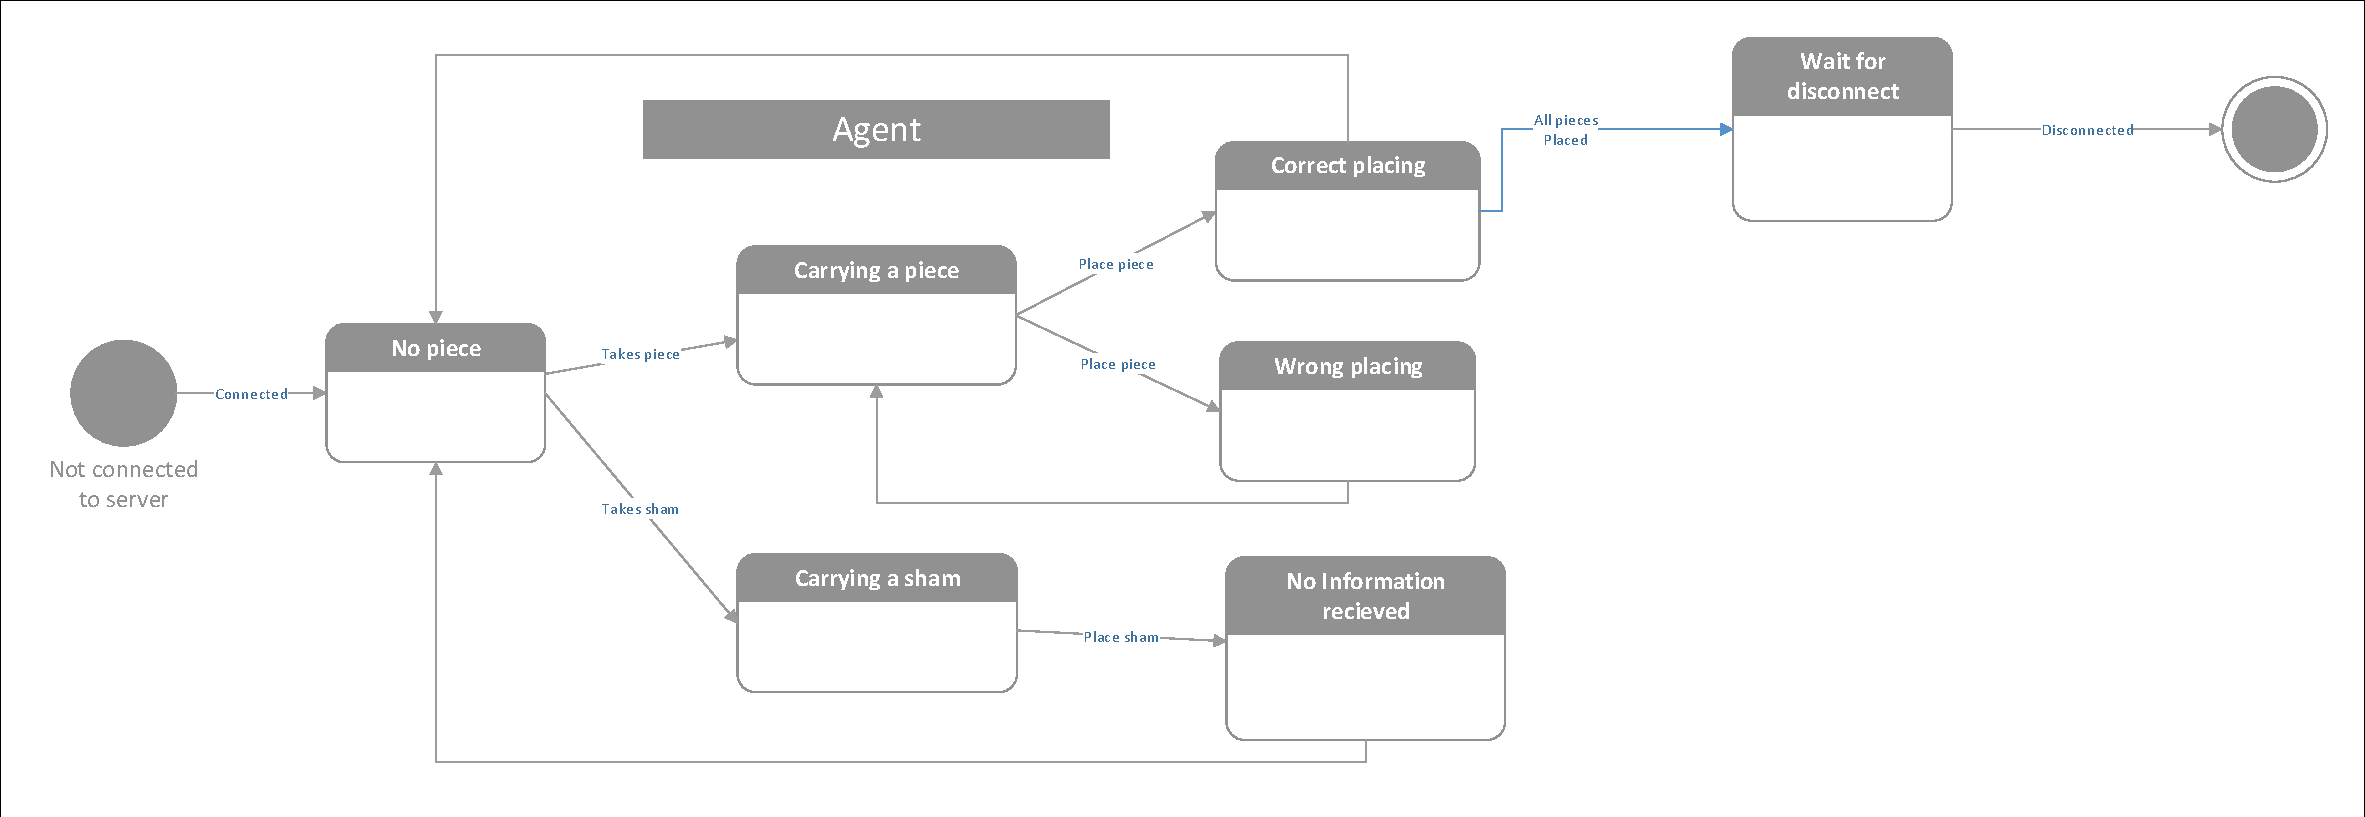
\includegraphics[scale=0.6]{Agent-state}
\caption{State diagram of agents}
\label{fig:AgentStateDiagram}
\end{center}


\end{sidewaysfigure}

\begin{figure}
\vspace*{-1.5in}
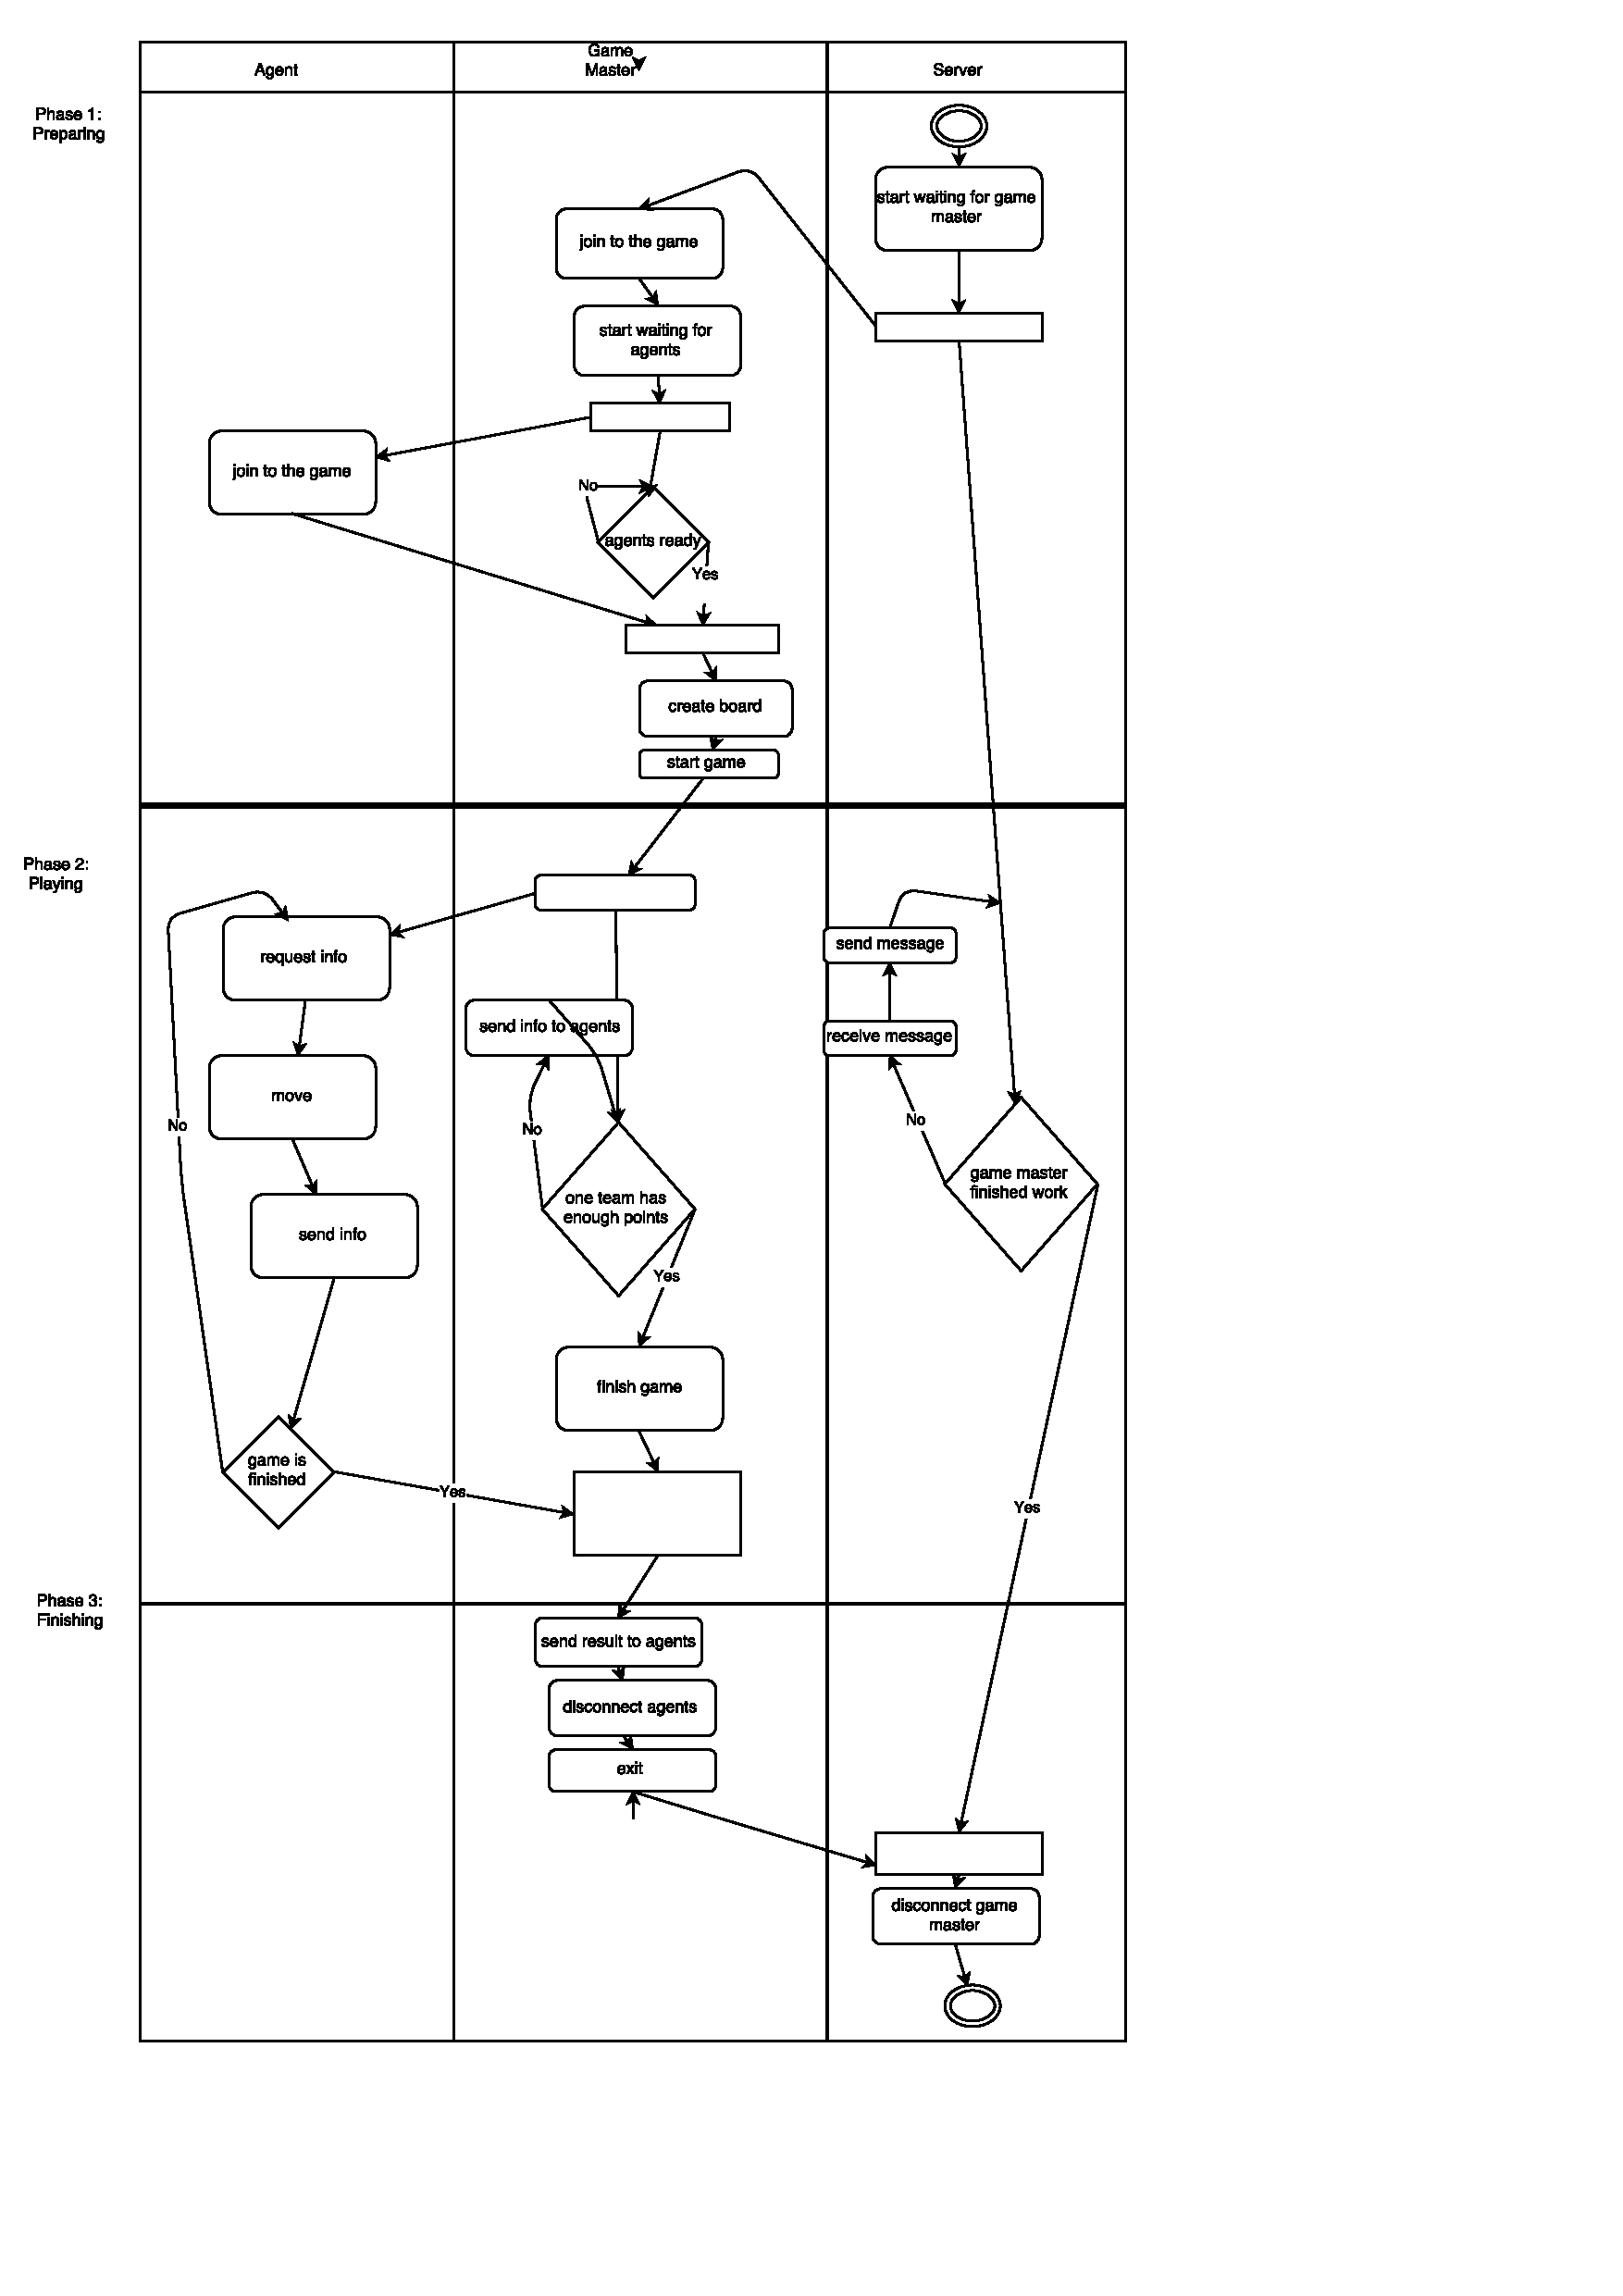
\includegraphics[scale=0.56]{active_diagram_5}
\caption{Activity Diagram}
\label{fig:ActiveDiagram}

\end{figure}

Figure \ref{fig:AgentStateDiagram} presents a state diagram from the point of view of an agent. \\

Agent actions have following ramifications and constrains:
\begin{itemize}


\item The piece is picked up by a Agent which moves into the piece’s field first.
\item Agent cannot move into a field occupied by another player.
\item Observing a field (either by discovering or entering it) results in receiving
information about the Manhattan distance to the nearest piece.
\end{itemize}

The Game Master may place a new piece to any field at any moment. The game finishes when one all pieces were collected by teams. The team which has collected more pieces(not sham) wins.
\subsection{Game interactions}
Each agent before moving sends information about move to the Game Master. The GM if the move is acceptable (no other agents on field, etc.) tells the agent that it's OK and updates game info. Else it sends deny to the agent. 

The agent may request information from another agent. If it succeeds, it receives all info known to that agent.\\

Figure \ref{fig:ActiveDiagram} presents activity diagram for an agent and Game Master.

\subsection{Configuration}



\newpage
\subsection{Ways of handling basic program errors}
\subsubsection{Loss of connection}

\begin{center}
{\bf Loss of connection with Agent}\\
\end{center}

\\{\bf Agent side}\\
When Agent loss connection with Game Master he does not perform moves in game and tries to reconnect with server.
\\{\bf Game Master side}\\
When Game Master recognizes that he can not comunicate with Agent, he only preserves Agent state, from other agent's point of view it looks like disconnected Agent does not perform any moves.

\begin{center}
\\{\bf Loss of connection with Game Master}\\
\end{center}
\\{\bf Agents side}\\
Agents no longer make moves and they only pings Game Master to check if he reconnected, after succesful reconnection they resume game.

\\{\bf Game Master side}\\
Game Master tries to reconnect to Server, after specified number of atempts to reconnect GM should give up.


\begin{center}
\\{\bf Loss of connection with Server}\\
\end{center}

\\{\bf Agents side}\\
They stop making their moves and start reconnection atempts.

\\{\bf Game Master side}\\
The same on Game Master side, GM preserves game state and tries to reconnect to server.


\section{Glossary}


\end{document}